\section{\textsc{Omlett ToMo}}

\subsection*{Zutaten für 1 Omlett:}

\begin{tabular}{p{7.5cm} p{7.5cm}}
	& \\
	4 Eier & 5 Cherrytomaten \\
	2TL Butter & 200g Mozzarella \\
	Salz & Pfeffer \\
	Basilikum nach Geschmack &
\end{tabular}

\subsection*{Serviervorschlag:}

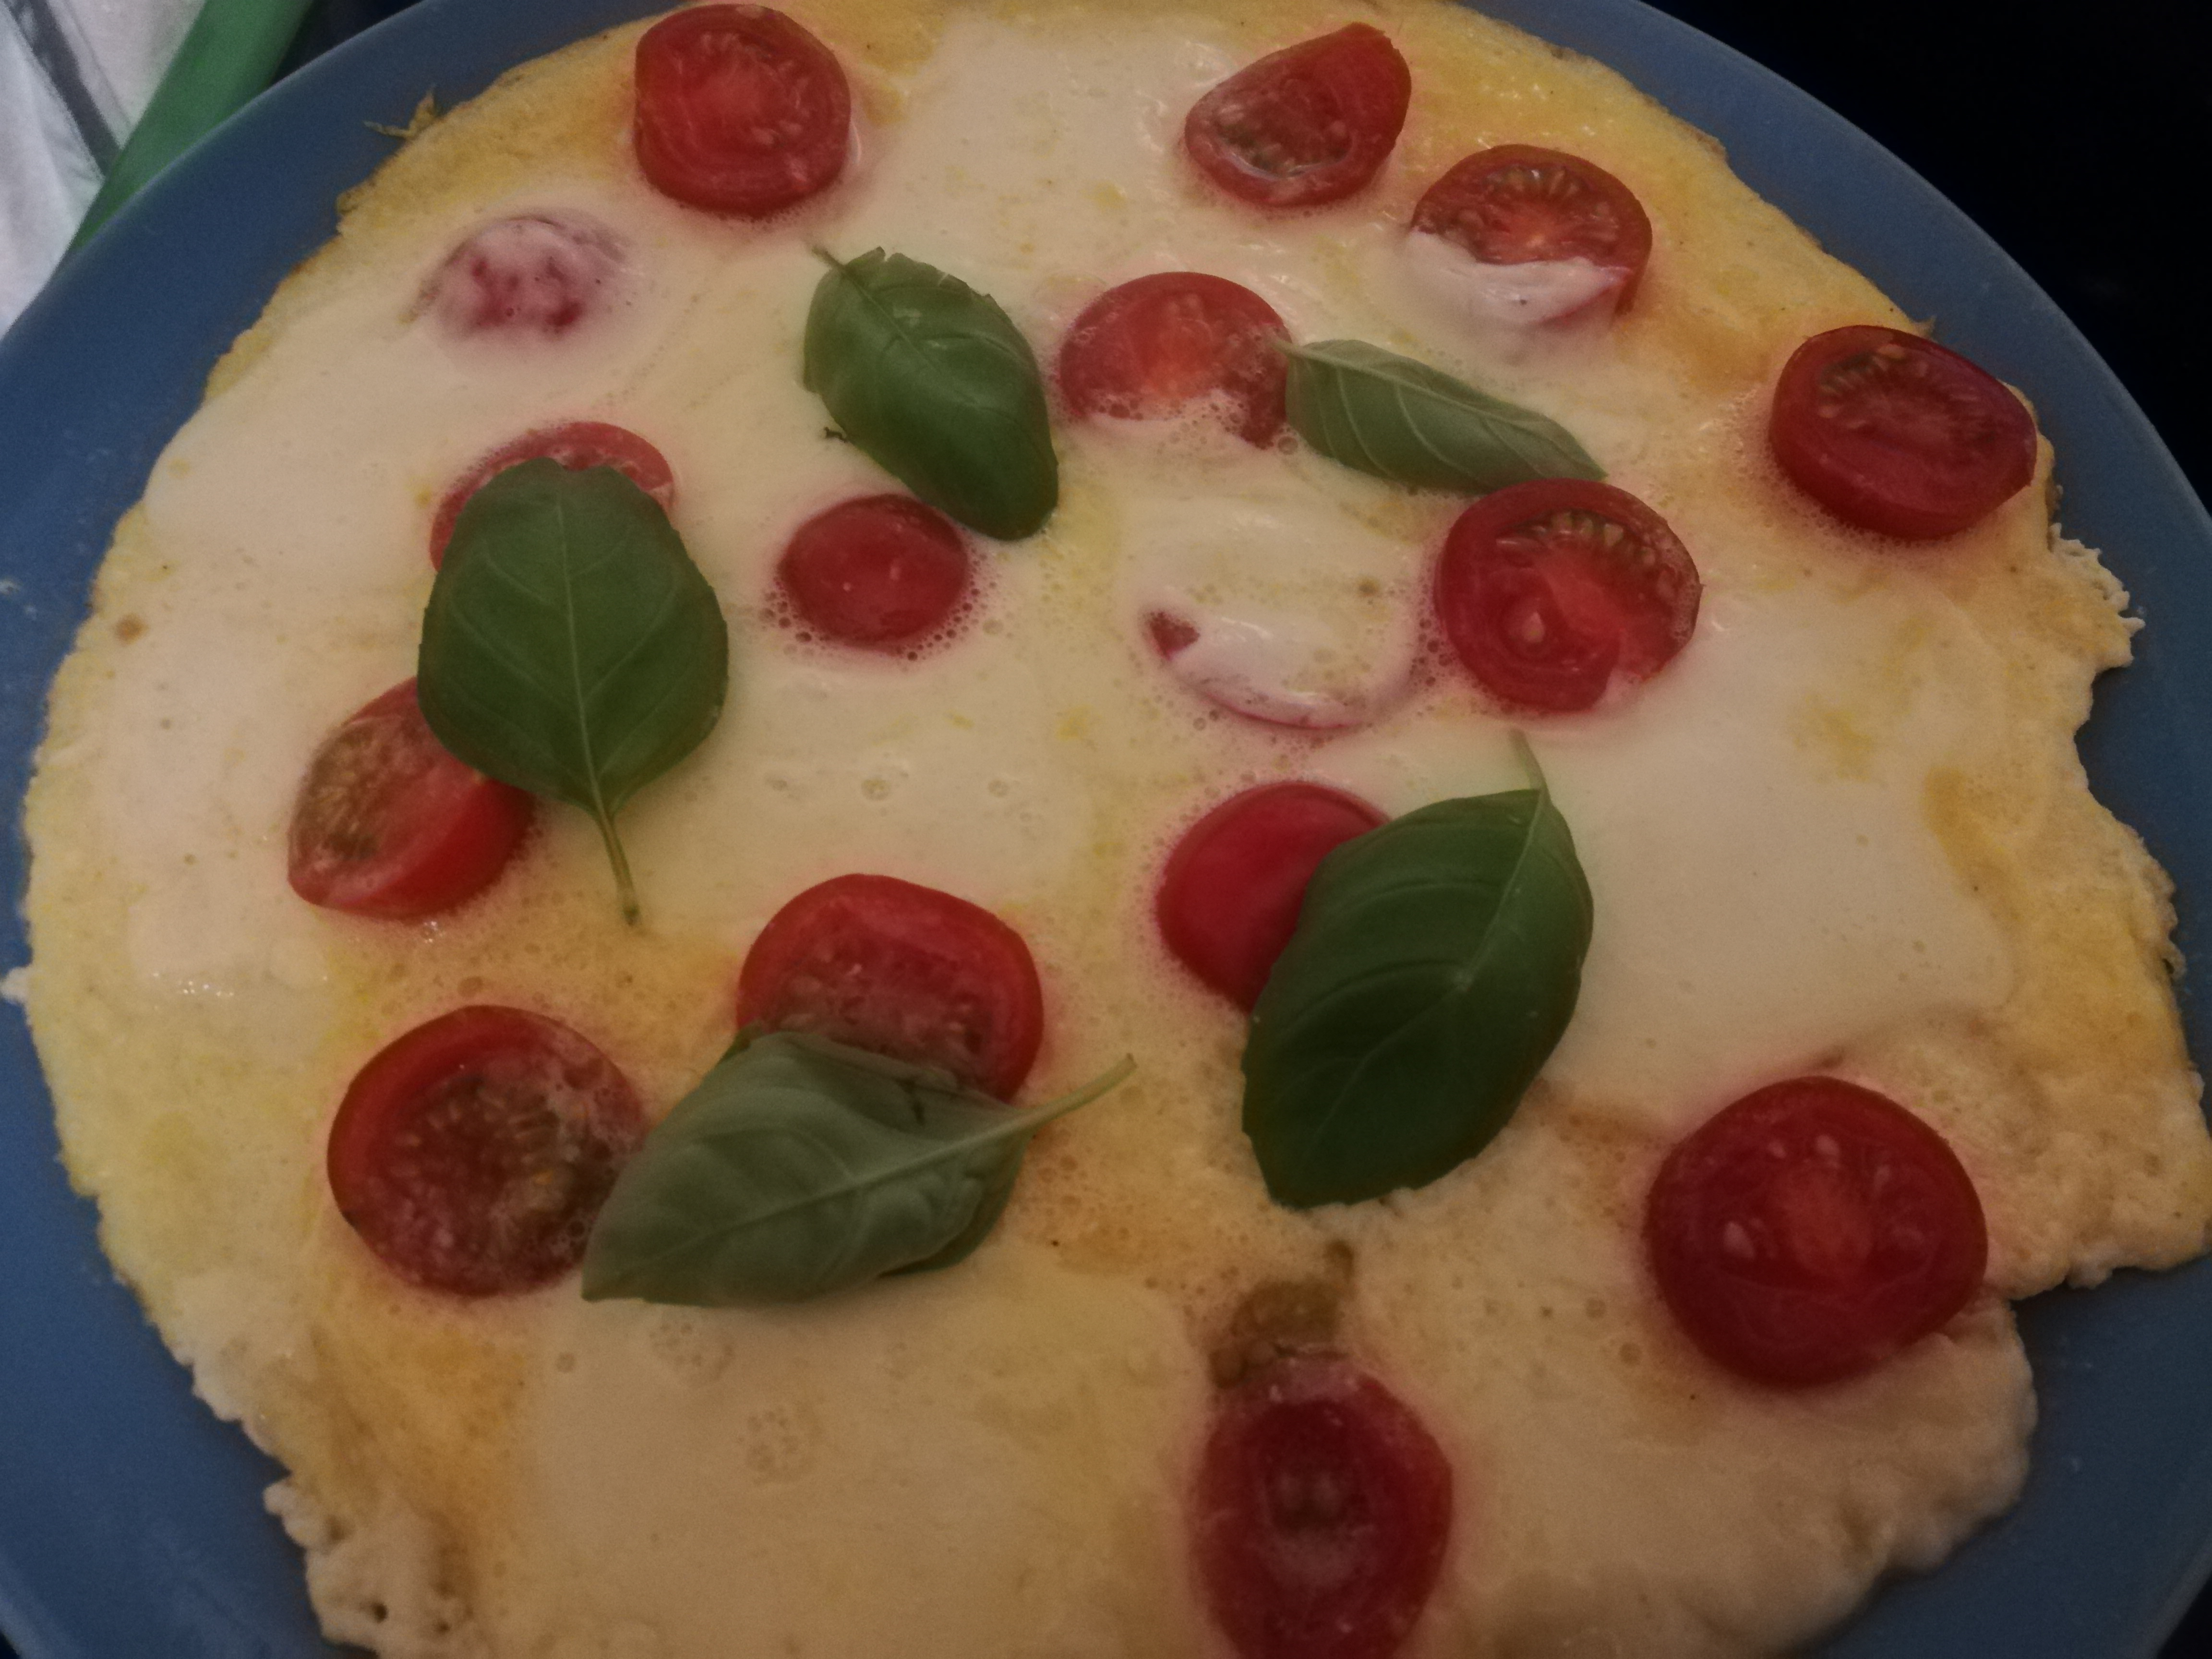
\includegraphics[width=\textwidth]{img/omlett/omlett_tomo_fertig.jpg}

\subsection*{So geht's:}

\begin{tabular}{p{15cm}}
	\\
	Die Eier mit einem Schneebesen schaumig schlagen.\\
	Salz und Pfeffer nach Belieben hinzufügen.\\
	Die Butter in einer Pfanne schmelzen lassen.\\
	Die Eimasse in die Pfanne geben und auf großer Hitze stocken lassen.\\
	Den Mozzarella und die Tomaten darauf verteilen.\\
	Mit einem Deckel auf kleiner Flamme 5min braten lassen.\\
	Auf einen großen Teller geben und mit dem Basilikum dekorieren.\\
\end{tabular}
